\documentclass[11pt]{article}
\usepackage[letterpaper,margin=0.9in]{geometry}
\usepackage[T1]{fontenc}
\usepackage{lmodern,amsmath,amssymb,amsthm,mathtools,microtype,tikz,enumitem,booktabs,xurl}
\usepackage[colorlinks=true,linkcolor=black,citecolor=black,urlcolor=blue!45!black]{hyperref}
\setlength{\parindent}{0pt}
\setlength{\parskip}{5pt plus 1pt minus 1pt}
\setlength{\emergencystretch}{2em}
\setlist{nosep,leftmargin=1.5em,topsep=4pt}
\newtheorem{theorem}{Theorem}[section]
\newtheorem{lemma}[theorem]{Lemma}
\newtheorem{proposition}[theorem]{Proposition}
\newtheorem{corollary}[theorem]{Corollary}
\theoremstyle{definition}
\newtheorem{definition}[theorem]{Definition}
\newcommand{\Z}{\mathbb Z}
\newcommand{\R}{\mathbb R}
\newcommand{\intr}{\operatorname{int}}
\newcommand{\dist}{\operatorname{dist}}
\newcommand{\lcm}{\operatorname{lcm}}
\hypersetup{pdfauthor={Daniel Wang and Peyton Wang}}

\title{Illumination in rectangular-spine combs}
\author{Daniel Wang \and Peyton Wang}
\date{Working draft v0.1 --- November 8, 2026}
\begin{document}\maketitle
\begin{abstract}
Let a polygon consist of a rectangular spine and finitely many disjoint rectangular teeth on one side. We prove that every pair of distinct interior points lying in the spine or on tooth middle rows is joined by a finite specular trajectory avoiding every polygon corner. All dimensions and marked points may be arbitrary real numbers, and there is no bound on the number of teeth. The main step is a monotone floor-matching iteration that terminates after finitely many steps at a point away from every aperture endpoint. For integer-coordinate teeth of height two, the theorem covers every pair of interior even-even lattice points. It does not cover arbitrary off-middle-row points in teeth.
\end{abstract}

\section{Geometry and statement}
A legal billiard path is a finite polygonal path with equal-angle reflections at smooth boundary points, with no contact with a genuine polygon corner. Two distinct interior points \emph{illuminate} one another if such a path connects them. Corners include convex corners; an artificial cut inside a room is not a mirror.

Fix a spine $[0,c]\times[y_-,y_+]$, where $c>0$, and finitely many right teeth
\[
 [c,R_j]\times[\ell_j,u_j],\qquad R_j>c,\quad \ell_j<u_j.
\]
Their vertical bands are separated by positive gaps and lie in $[y_-,y_+]$. A tooth may share the global floor or ceiling. Assume their union $P$ is a strictly simple polygonal disk. Let $E$ be the interior points that either have $x\le c$ or lie on a tooth's middle horizontal line.

\begin{theorem}\label{thm:comb}
Every distinct pair in $E$ illuminates. The dimensions, tooth depths and marked points may be arbitrary real numbers; the number of teeth is unrestricted.
\end{theorem}

The interest is the absence of a size or wall-count cap. Additional teeth do not enter the selected path. The middle-row hypothesis is essential to the argument: it makes the two signs of a genuine unfolded endpoint combine into one half-period progression.

\begin{figure}[htbp]\centering
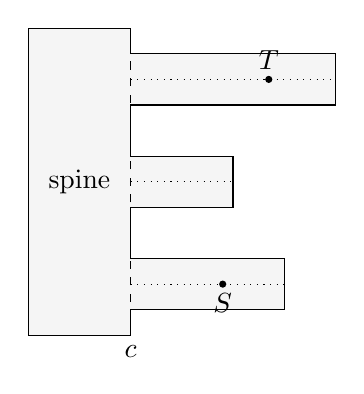
\begin{tikzpicture}[scale=.65]
\filldraw[fill=gray!8] (0,0)--(2,0)--(2,.5)--(5,.5)--(5,1.5)--(2,1.5)--(2,2.5)--(4,2.5)--(4,3.5)--(2,3.5)--(2,4.5)--(6,4.5)--(6,5.5)--(2,5.5)--(2,6)--(0,6)--cycle;
\draw[dashed] (2,0)--(2,6);
\draw[dotted] (2,1)--(5,1) (2,3)--(4,3) (2,5)--(6,5);
\fill (3.8,1) circle(2pt) node[below]{$S$};
\fill (4.7,5) circle(2pt) node[above]{$T$};
\node at (1,3){spine};\node[below] at (2,0){$c$};
\end{tikzpicture}
\caption{A rectangular-spine comb. The dotted lines are tooth middle rows; the dashed spine edge contains open mouths and boundary gaps. The drawing illustrates the endpoint class, not a specific computed trajectory.}
\end{figure}

\section{A finite matching lemma}
Take two selected teeth, ordered vertically, with bands $[0,u]$ and $[H-v,H]$, where $u,v,c>0$ and $H>u+v$. Write the actual marks as
\[
 S=(c+D_s,u/2),\qquad T=(c+D_t,H-v/2),\qquad D_s,D_t>0.
\]
Each far wall lies strictly beyond its mark. Set $A=D_s+D_t+2c$ and, for $\tau\ge0$, define
\begin{align*}
 n_s(\tau)&=\left\lfloor D_s\tau/u+1/2\right\rfloor,&
 n_t(\tau)&=\left\lfloor D_t\tau/v+1/2\right\rfloor,\\
 \Phi(\tau)&=\frac{H-(u+v)/2+u n_s(\tau)+v n_t(\tau)}{A}.
\end{align*}

\begin{lemma}\label{lem:matching}
Iteration from $\tau_0=0$ by $\tau_{j+1}=\Phi(\tau_j)$ stops after finitely many steps at $\tau>0$. At this value,
\begin{gather*}
 r_s=D_s\tau+u/2-u n_s(\tau)\in(0,u),\qquad
 r_t=D_t\tau+v/2-v n_t(\tau)\in(0,v),\\
 r_s+r_t+2c\tau=H.
\end{gather*}
\end{lemma}
\begin{proof}
The function $\Phi$ is nondecreasing and $\Phi(0)>0$. Since $\lfloor x\rfloor\le x$,
\[
 \Phi(\tau)\le \frac{H+(D_s+D_t)\tau}{A}.
\]
Thus $\Phi(H/(2c))\le H/(2c)$. All iterates lie in $[0,H/(2c)]$ and are nondecreasing. The two floor functions have finite ranges on that interval, so $\Phi$ has finite range there. The iteration must become stationary.

Let $j$ be the first index with $\Phi(\tau_j)=\tau_j$. Then $j\ge1$ and $\tau_{j-1}<\tau_j$. If $n_s$ jumps at $\tau_j$, its value exceeds $n_s(\tau_{j-1})$ by at least one, and $n_t$ cannot decrease. Hence
\[
 \Phi(\tau_j)\ge\Phi(\tau_{j-1})+u/A>\tau_j,
\]
which is impossible. The same argument excludes a jump of $n_t$, including simultaneous jumps. The remainders lie in $[0,u)$ and $[0,v)$ by definition; equality at zero is exactly a jump. They are therefore strict. Substitution of the fixed-point equation gives the last identity.
\end{proof}

\section{An actual path between different teeth}
For the selected integers, write $n_s=2k_s$ or $2k_s+1$, and set $\sigma_s=1$ in the first case, $\sigma_s=-1$ in the second. Then
\[
 r_s=\sigma_s u/2+D_s\tau-2uk_s,\qquad k_s=\lfloor n_s/2\rfloor\ge0.
\]
These are genuine source images of an endpoint at height $u/2$. The analogous identity holds for $r_t$. For an off-middle endpoint, this half-period replacement would not be valid.

Launch left from $S$, with initial vertical sign $\sigma_s$ and absolute slope $\tau$. In its tooth chart the initial ordinate is $\sigma_su/2$ and the final ordinate at $x=c$ is $2uk_s+r_s$. Horizontal-wall contacts occur at
\[
 x_j=c+D_s-\frac{ju-\sigma_su/2}{\tau},
 \qquad y_j=\begin{cases}u&j\text{ odd},\\0&j\text{ even}.\end{cases}
\]
For $\sigma_s=1$, use $j=1,\ldots,2k_s$; for $\sigma_s=-1$, use $j=0,\ldots,2k_s$. All contact times are positive. Because $0<r_s<u$, the last contact precedes the mouth and every $x_j$ is strictly greater than $c$. Contacts are strictly left of the source and far wall, hence are smooth points of the actual tooth walls. After $n_s$ reflections the ray reaches $(c,r_s)$ moving upward.

Join this mouth to the upper mouth $(c,H-r_t)$ through
\[
 M=(0,r_s+c\tau).
\]
The identity in Lemma~\ref{lem:matching} makes the two spine legs have slopes $-\tau$ and $\tau$, with one ordinary reflection at $M$. The height of $M$ lies strictly between the two mouth heights, hence strictly between the global floor and ceiling. Both open legs have $x<c$ and avoid all other teeth and mouths. A reflected reverse of the upper-tooth construction reaches the actual $T$ with matching velocity.

There are $n_s+n_t+1$ reflections. No artificial spine cut acts as a mirror. The source tooth, open spine and target tooth are traversed in that order; the last tooth segment reaches $T$ itself. Reversal handles either ordering of the marks.

\section{One spine point and one tooth point}
Let $S=(x_s,y_s)$ satisfy $0<x_s\le c$ and $y_-<y_s<y_+$, and let
\[
 T=(c+D,\ell+u/2),\qquad D>0.
\]
If $y_s\in[\ell,\ell+u]$, the direct segment lies inside the spine before the mouth and strictly within the selected tooth afterwards. Actual interiority rules out a genuine corner at a seam endpoint.

Otherwise reflect $S$ in the actual left wall, obtaining $(-x_s,y_s)$, and set $C=c+x_s>0$. The legitimate middle-row target images have ordinates $\ell+u/2+un$, $n\in\Z$. Their lines from the source image have slopes and mouth heights
\[
 \tau_n=\frac{\ell+u/2+un-y_s}{C+D},\qquad z_n=y_s+C\tau_n.
\]
The values $z_n$ form a two-sided arithmetic progression with spacing $Cu/(C+D)<u$. Equivalently, the open interval of admissible integers $n$ has length $(C+D)/C>1$. Select $n$ with $\ell<z_n<\ell+u$.

The left-wall contact height $y_s+x_s\tau_n$ is strictly between $y_s$ and $z_n$, since $0<x_s<C$. It is a smooth actual wall point. The two spine legs stay within the spine. After the strict mouth, every tooth-wall reflection occurs with $x>c$ and before the actual target abscissa. The selected target image folds to the actual height $\ell+u/2$ for either parity of $n$; negative $n$ and either sign of slope are legitimate finite unfoldings. This also handles a source on the seam $x=c$ of another mouth: its first leg enters the spine.

\section{Exhaustion and the lattice corollary}
Two points in one tooth are directly visible. Two spine points with at least one abscissa strictly less than $c$ are directly visible. If both lie on different mouth seams $x=c$, use the left-wall reflection
\[
 (0,(y_s+y_t)/2).
\]
Its two open legs have $x<c$, and its contact is smooth because both endpoint heights lie strictly inside the global vertical range. This avoids travel along boundary gaps of $x=c$. These cases and the preceding sections exhaust every distinct pair in $E$, proving Theorem~\ref{thm:comb}.

\begin{corollary}
Suppose the comb has integer axial boundary coordinates and every tooth has height two. Every distinct pair of actual interior points in $(2\Z)^2$ illuminates, with no bound on walls, area, tooth count, depth or lattice diameter.
\end{corollary}
\begin{proof}
An interior even-even point outside the spine must have an even integer ordinate strictly between $\ell_j$ and $\ell_j+2$. If $\ell_j$ is even there is none; if it is odd the only possibility is the middle row $\ell_j+1$. All other such points are in the spine or its mouth seams. Apply the theorem.
\end{proof}

\section{Scope and source record}
The theorem is an analytic existence proof. Finite examples can check the formulas but do not establish the real-parameter quantifiers. Arbitrary off-middle-row tooth endpoints, two-sided combs and mixed diagonal walls require separate arguments. In particular, this paper makes no general minimum-wall claim.

The complete underlying argument is \texttt{midheight-comb-proof.md} in the repository's \path{research/illumination-generalization-2026-11-06/construction/} directory. Its later scoped acceptance is \texttt{midheight-comb-independent-acceptance.json} in the neighboring \texttt{review/} directory. The accompanying \texttt{provenance.json} identifies those source versions. The distinct two-sided lattice comb results remain indexed in result R05; they are not additional conclusions of this theorem. This working draft has not been externally refereed or formalized in a proof assistant.

\smallskip\noindent\textbf{Acknowledgments.} The authors used AI tools, including OpenAI Codex and Anthropic Claude, to develop and revise this research, its theorem proofs, and the manuscript. The authors remain responsible for the content.
\end{document}
